\documentclass[t,usenames,dvipsnames]{beamer}
\usetheme{CambridgeUS}
\usecolortheme{dolphin}

\usepackage[T1]{fontenc}
\usepackage{amsfonts,amssymb,amsmath,amsthm,mathrsfs,stmaryrd,amstext}

% you probably need to load these
\usepackage{tikz}
	\usetikzlibrary{calc}

\definecolor{pal1}{RGB}{199,53,88}
\definecolor{pal2}{RGB}{225,127,91}
\definecolor{pal4}{RGB}{102,211,100}
\definecolor{pal5}{RGB}{57,213,172}
\definecolor{pal6}{RGB}{75,159,190}
\definecolor{pal7}{RGB}{113,103,188}

\begin{document}

\begin{frame}[plain]
\centering
\begin{tikzpicture}[>=stealth,scale=.7]
	\begin{scope}[shift={(-6,0)},line width=1pt]
		\node[anchor=south] at (0,3) {$A$};
		\draw (0,0) circle (2 and 3);
		\coordinate (a1) at (-.6,1.9);
		\coordinate (a2) at (.5,.4);
		\coordinate (a3) at (-.1,-1.5);
		\only<1>{
			\filldraw[] (a1) circle (3pt and 3pt);		
		}
		\only<2->{
			\filldraw[pal1] (a1) circle (3pt and 3pt);
		}
		\only<1,3->{
			\filldraw[] (a2) circle (3pt and 3pt);
			\filldraw[] (a3) circle (3pt and 3pt);
		}
		\only<2>{
			\filldraw[pal6] (a2) circle (3pt and 3pt);
			\filldraw[pal4] (a3) circle (3pt and 3pt);
		}
	\end{scope}
	\begin{scope}[shift={(0,0)},line width=1pt]
		\node[anchor=south] at (0,3) {$B$};
		\draw (0,0) circle (2 and 3);
		\coordinate (fa1) at (-.4,1.2);
		\coordinate (fa2) at (.5,.5);
		\coordinate (fa3) at (0,-1.8);
		\coordinate (fa1t) at ($(fa1) + (.1,.6)$);
		\coordinate (fa2t) at ($(fa2) + (.1,-.7)$);
		\coordinate (fa3t) at ($(fa3) + (-.25,-.4)$);
		\coordinate (fa1s) at ($(fa1) + (1,.2)$);
		\only<2->{
			\draw[pal1,rotate=-15] (fa1) circle (1 and 1.2);
		}
		\only<2>{
			\draw[pal6,rotate=10] (fa2) circle (1 and 1.2);
			\draw[pal4,rotate=2] (fa3) circle (1.1 and .9);
		}
		\coordinate (b1) at (-.9,1.3);
		\coordinate (b2) at (0,.8);
		\coordinate (b3) at (.8,.2);
		\coordinate (b4) at (-.8,-1.6);
		\coordinate (b5) at (-.1,-2.2);
		\coordinate (b6) at (.5,-1.3);
		\coordinate (bx) at (1.2,-1);
		\only<1,2,6>{
			\filldraw[] (b1) circle (3pt and 3pt);
			\filldraw[] (b2) circle (3pt and 3pt);
		}
		\only<3-4>{
			\filldraw[pal5] (b1) circle (3pt and 3pt);
			\filldraw[pal2] (b2) circle (3pt and 3pt);
		}
		\only<1-4,6>{
			\filldraw[] (b3) circle (3pt and 3pt);
			\filldraw[] (b4) circle (3pt and 3pt);
			\filldraw[] (b5) circle (3pt and 3pt);
			\filldraw[] (b6) circle (3pt and 3pt);
			\filldraw[] (bx) circle (3pt and 3pt);
		}
		\only<5>{
			\filldraw[gray!50!white] (b1) circle (3pt and 3pt);
			\filldraw[gray!50!white] (b2) circle (3pt and 3pt);
			\filldraw[gray!50!white] (b3) circle (3pt and 3pt);
			\filldraw[gray!50!white] (b4) circle (3pt and 3pt);
			\filldraw[gray!50!white] (b5) circle (3pt and 3pt);
			\filldraw[gray!50!white] (b6) circle (3pt and 3pt);
			\filldraw[gray!50!white] (bx) circle (3pt and 3pt);
		}
	\end{scope}
	\begin{scope}[shift={(6,0)},line width=1pt]
		\node[anchor=south] at (0,3) {$C$};
		\draw (0,0) circle (2 and 3);
		\coordinate (gb1) at (0,1.2);
		\coordinate (gb2) at (.3,0);
		\coordinate (gb1t) at ($(gb1) + (-.1,.4)$);
		\coordinate (gb2t) at ($(gb2) + (-.1,-.3)$);
		\coordinate (gb12) at (0,.5);
		\coordinate (gb12t) at ($(gb12) + (-.8,-.5)$);
		\only<3-5>{
			\draw[pal5] (gb1) circle (1.3 and 1.1);
			\draw[pal2,rotate=10] (gb2) circle (1 and 1.2);
		}
		\only<4-5>{
			\draw[pal1,dashed] (gb12) circle (1.7 and 2.1);
		}
		\only<6->{
			\draw[pal1] (gb12) circle (1.7 and 2.1);
		}
		\coordinate (c1) at (-.7,1.3);
		\coordinate (c2) at (.6,1.4);
		\coordinate (c3) at (.1,.7);
		\coordinate (c4) at (.4,-.4);
		\coordinate (cx) at (-.6,-2.1);
		\coordinate (cy) at (.6,-2.2);
		\only<1-4,6>{
			\filldraw[] (c1) circle (3pt and 3pt);
			\filldraw[] (c2) circle (3pt and 3pt);
			\filldraw[] (c3) circle (3pt and 3pt);
			\filldraw[] (c4) circle (3pt and 3pt);
			\filldraw[] (cx) circle (3pt and 3pt);
			\filldraw[] (cy) circle (3pt and 3pt);
		}
		\only<5>{
			\filldraw[gray!50!white] (c1) circle (3pt and 3pt);
			\filldraw[gray!50!white] (c2) circle (3pt and 3pt);
			\filldraw[gray!50!white] (c3) circle (3pt and 3pt);
			\filldraw[gray!50!white] (c4) circle (3pt and 3pt);
			\filldraw[gray!50!white] (cx) circle (3pt and 3pt);
			\filldraw[gray!50!white] (cy) circle (3pt and 3pt);
		}
	\end{scope}
	\only<2->{
		\draw[pal1,->,shorten <=5pt, shorten >=5pt,line width=.8pt] (a1) to[out=35,in=140] (fa1t);
	}
	\only<2>{
		\draw[pal6,->,shorten <=5pt, shorten >=5pt,line width=.8pt] (a2) to[out=-40,in=-160] (fa2t);
		\draw[pal4,->,shorten <=5pt, shorten >=5pt,line width=.8pt] (a3) to[out=-20,in=-170] (fa3t);
	}
	\only<3-4>{
		\draw[pal5,->,shorten <=5pt, shorten >=5pt,line width=.8pt] (b1) to[out=50,in=140] (gb1t);
		\draw[pal2,->,shorten <=5pt, shorten >=5pt,line width=.8pt] (b2) to[out=30,in=190] (gb2t);
	}
	\only<5>{
		\draw[pal1,->,shorten <=5pt, shorten >=5pt,line width=.8pt,dashed] (fa1s) to[out=-5,in=190] (gb12t);
	}
	\only<6>{
		\draw[pal1,->,shorten <=5pt, shorten >=5pt,line width=.8pt] (fa1s) to[out=-5,in=190] (gb12t);
	}
	
	% functions
	\only<2->{
		\node at (-3,-4) {$f : A \to \mathcal{P}(B)$};
	}
	\only<3-4>{
		\node at (3,-4) {$g : B \to \mathcal{P}(C)$};
	}
	\only<5->{
		\node at (3,-4) {$\mathcal{P}(g) : \mathcal{P}(B) \to \mathcal{P}(\mathcal{P}(C))$};
	}
	\only<5>{
		\node at (0,-5.1) {$f;\mathcal{P}(g) : A \to \mathcal{P}(\mathcal{P}(C))$};
	}
	\only<6>{
		\node at (0,-5.1) {$f;\mathcal{P}(g);\mu_C : A \to \mathcal{P}(C)$};
	}
\end{tikzpicture}
\end{frame}

\end{document}